\documentclass{article}
\usepackage{graphicx}
\begin{document}
\section*{Simulating random walks}
Imagine you need to follow a straight line home from some point P. As you have
a lot of time on your hands, you decide to this by taking a step forward or 
backward based on some random event -- say, flipping a coin. Since you are equally
likely to take a step forward or backward, you might expect never to reach home. 
But here's the cool part -- it is \textbf{mathematically certain} that you will reach
your destination in a \emph{finite} amount of time.
\newline \\ A good way to test these kind of theories is to run \emph{simulations}
on a computer. Computers are good at generating seemingly random numbers:
\begin{figure}[h]
\begin{center}
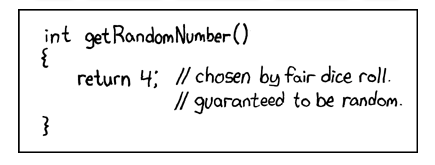
\includegraphics[height=80pt]{../pictures/xkcd_random.png}
\end{center}
\end{figure}
\\ Simulate a random walk using the \texttt{numpy.random} module. A
one dimensional random walk might look like this:
\begin{figure}[h]
\begin{center}
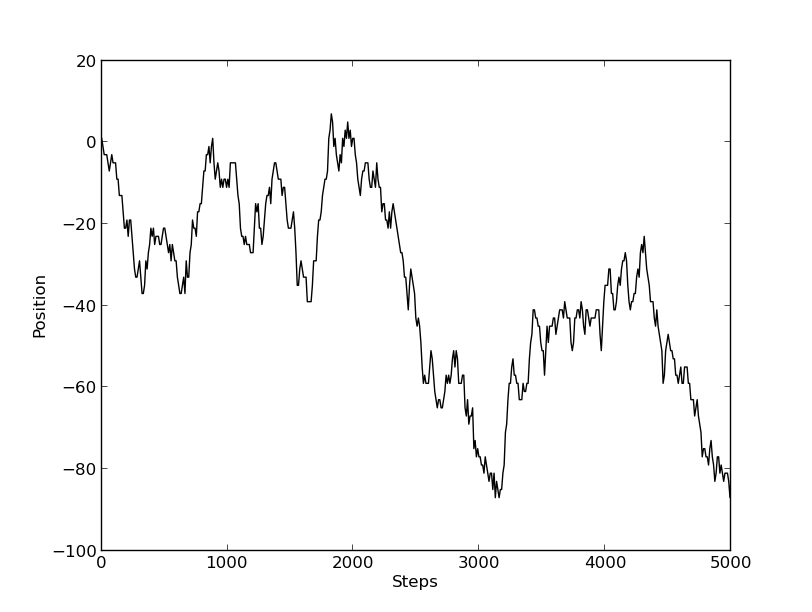
\includegraphics[height=180pt]{../pictures/randomwalk.png}
\end{center}
\end{figure}
\\ This may not be a very exciting figure, but if you run several simulations
like these, some very interesting features start to pop up. Put your code in a
loop so that your program simulates \textbf{N} random walks. Once you have this 
running, you can arrive at all sorts of interesting conclusions and experiment with
different parameters.
\end{document}

